\section{Generowanie raportu}

Końcowym etapem działania jest możliwość wygenerowania finalnego raportu w formacie arkusza kalkulacyjnego na podstawie uzupełnionej bazy danych. W związku z tym w Power Apps przygotowano mechanizm łączący dane z trzech list sharepointowych, które następnie są przesyłane do Power Automate, gdzie podlegają dalszemu przetwarzaniu. Wynikiem tego jest kompletny arkusz Excel, który jest zapisywany na platformie SharePoint.

\subsection{Łączenie źródeł danych do formy docelowej}

Pierwszym krokiem do wygenerowania gotowego raportu jest konsolidacja potrzebnych danych w odpowiedniej formie. Do tego celu zaimplementowano ekran przedstawiony na rysunku \ref{fig:generateraportform}. Składa się on z dwóch formularzy -- węższy po lewej stronie oraz szerszy po prawej. W pierwszym z nich znajdują się dwa
pola wyboru typu \emph{Dropdown}, w których należy wybrać numer indykacji oraz roku do pobrania danych z list, natomiast w drugiej widnieje podgląd zawartości danych do wygenerowania w formie tabeli, która może zostać przekazana do Power Automate.

\begin{figure}[H]
    \centering
    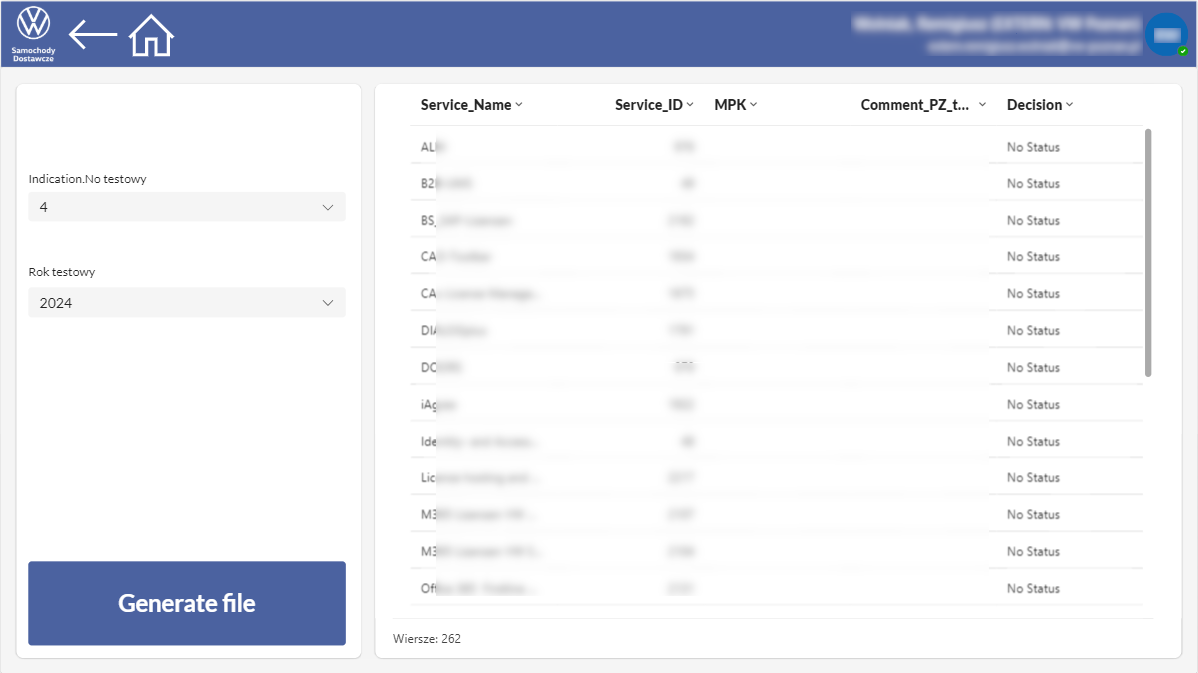
\includegraphics[width=0.9\textwidth]{figures/GenerateRaportForm.png}
    \caption{Ekran generowania raportu}
    \label{fig:generateraportform}
\end{figure}

Zebrane dane przechowywane są w tymczasowej kolekcji \textit{CombinedData}, która składa się z informacji z trzech źródeł, odpowiednio dopasowanych do wybranego przez użytkownika roku oraz indykacji. Przykładowy fragment kodu odpowiedzialnego za tworzenie tej kolekcji przedstawiono w listingu~\ref{lst:combineddata}:

\begin{lstlisting}[language=PowerFx, caption={Fragment kodu tworzącego kolekcję CombinedData}, label={lst:combineddata}] 
    ClearCollect(
    CombinedData;
    AddColumns(
        LocalServiceData;
        MPK;
        LookUp(
            LocalCostData;
            Service_ID = LocalServiceData[@Service_ID] && Year = Year_Dropdown_1.Selected.Value;
            MPK
        );
        Comment_PZ_to_WOB;
        LookUp(
            LocalIndicationsData;
            Service_ID = LocalServiceData[@Service_ID] && Year = Year_Dropdown_1.Selected.Value && IndicationNo = IndicationNo_Dropdown_1.Selected.Value;
            Comment_PZ_to_WOB);     
    [...]
);;

\end{lstlisting}

W fragmencie kodu przedstawiono wykorzystanie funkcji \textit{LookUp}, która pozwala na pobranie danych z różnych kolekcji na podstawie określonych kryteriów. Przykładowo, pierwsze wywołanie \textit{LookUp} dopasowuje dane z tabeli \textit{LocalCostData}

\subsection{Przekazywanie danych do Power Automate}

W lewym dolnym rogu interfejsu znajduje się przycisk \textit{Generate file}, który po naciśnięciu uruchamia \textit{flow} w Power Automate, odpowiedzialne za tworzenie pliku na podstawie danych wejściowych. Dane te są przekazywane do usługi Power Automate w postaci ciągu tekstowego, sformatowanego jako JSON\footnote{JSON - format wymiany danych, który jest oparty na strukturze tekstowej}, wykorzystując połączone informacje z trzech źródeł zawarte w kolekcji \textit{CombinedData}, dostosowane do wybranego przez użytkownika zestawu roku i indykacji. Kod wywołujący funkcję \textit{GenerateRaport} przedstawiono w listingu~\ref{lst:generateraport}.



\begin{lstlisting}[language=PowerFx, caption={Kod wywołujący funkcję GenerateRaport}, label={lst:generateraport}]
    GenerateRaport.Run(
        Substitute(
            "[" & 
            Concat(
                CombinedData;
                "{""Service_ID"":""" & Service_ID & """," &
                """Service_Name"":""" & Service_Name & """," &
                """MPK"":""" & MPK & """," &
                """Comment_PZ_to_WOB"":""" & Comment_PZ_to_WOB & """," &
                """Decision"":""" & Decision & """},"
            ) & 
            "]",
            "},]"; 
            "}]"
        ),
        IndicationNoCollect.Value,
        YearNoCollect.Value
    )
    \end{lstlisting}



\subsection{Generowanie raportu w Power Automate}


\emph{Flow} o nazwie \emph{GenerateRaport} składa się z kilku komponentów, które finalizują tworzenie gotowego raportu przekazywanego do zakładu w Wolfsburgu, takich jak:

\begin{itemize}
    \item \textbf{Wejście danych:} \emph{Flow} przyjmuje trzy dane wejściowe: ciąg znaków w formacie JSON, zawierający dane przekazane z aplikacji do przetworzenia, wybraną indykację oraz wybrany rok.
    \item \textbf{Inicjalizacja zmiennej:} W tym kroku tworzona jest zmienna odpowiedzialna za nazwę generowanego pliku. Zmienna zawiera dynamicznie generowaną datę utworzenia pliku, która w dalszej kolejności pozostanie niezmienna, niezależnie od czasu wykonania kolejnych instrukcji.
    \item \textbf{Generowanie pustego arkusza Excel:} Wykorzystywany jest statyczny plik Excel, zapisany w formacie Base64, który pełni rolę szablonu dla dalszego przetwarzania.
    \item \textbf{Tworzenie pliku na SharePoint:} Szablon arkusza zostaje zapisany w określonej lokalizacji w bibliotece SharePoint.
    \item \textbf{Sprawdzenie dostępności pliku:} W celu upewnienia się, że plik jest gotowy do dalszego przetwarzania, uruchamiana jest pętla \emph{Do until}, która weryfikuje dostępność pliku na platformie.
    \item \textbf{Uruchomienie skryptu:} Na końcu przepływu wywoływany jest skrypt \emph{OfficeScript}, który generuje finalny arkusz Excel. Arkusz ten zawiera pełne dane i jest gotowy do przekazania odbiorcy.
\end{itemize}

Schemat \ref{fig:generateflowcomponent} przedstawia szczegółowy schemat przepływu, uwzględniający poszczególne kroki oraz przepływ danych między nimi.

\begin{figure}[H]
    \centering
    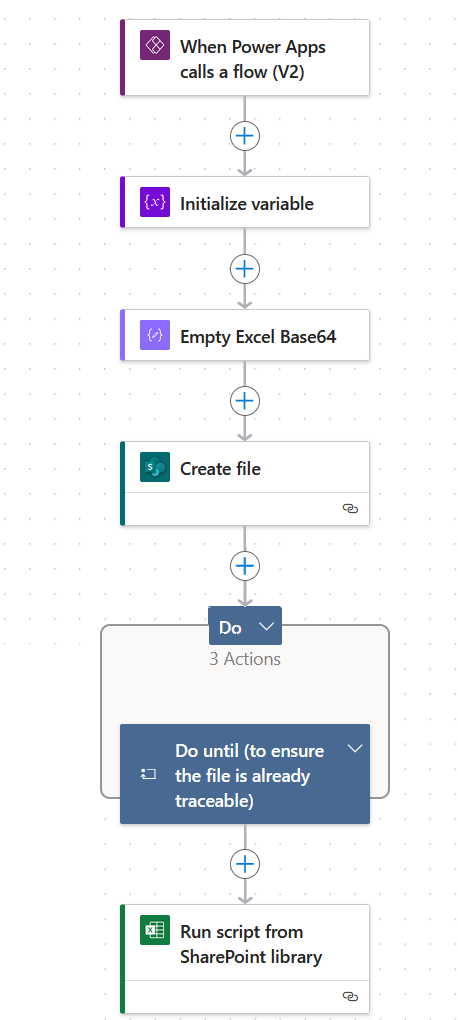
\includegraphics[width=0.45\textwidth]{figures/GenerateRaportFlow.png}
    \caption{Schemat przepływu \emph{GenerateRaport}}
    \label{fig:generateflowcomponent}
\end{figure}

\subsection{Opis działania skryptu generującego raport}

Skrypt odpowiedzialny za generowanie raportu wykonuje kilka operacji. Jego główne funkcje to:
\begin{itemize}
    \item \textbf{Parsowanie danych wejściowych:} Przyjęcie danych w formacie JSON oraz roku. W przypadku błędu parsowania JSONa, tworzy arkusz z odpowiednim komunikatem o błędzie.
    \item \textbf{Tworzenie arkusza:} Sprawdzenie, czy arkusz wynikowy już istnieje -- jeśli tak, to usuwa go i tworzy nowy o stałej nazwie.
    \item \textbf{Dynamiczne wstawianie danych:} Wprowadzenie dynamicznych wartości na podstawie roku, takich jak \texttt{PL<rok>} oraz \texttt{PLAN}, w odpowiednich komórkach.
    \item \textbf{Generowanie tabeli:} Tworzenie nagłówków tabel (np. \texttt{Service\_ID}, \texttt{Service\_Name}) oraz wprowadzenie danych wypełniające tabelę, pobierane z JSON-a.
    \item \textbf{Formatowanie:} Formatowanie komórek arkusza -- skrypt dodaje filtry oraz zmienia szerokość kolumn, co sprawia, że wygląd arkusza jest spójny z tymi tworzonymi do tej pory ręcznie.
\end{itemize}




